\chapter{Experimental setup}

One of the most useful methods to study the subatomic world of particle physics uses particle colliders. In such machines, particles are accelerated to very high speeds and energies, and smashed into each other. The particles that emerge from the collisions are then measured in a particle detector and then studied and analyzed. At the time of writing this thesis, the world's largest and highest-energy collider to date is the \gls{lhc} located in Geneva, Switzerland, operated by the \gls{cern}. For the present work, data from the \gls{cms} experiment has been analyzed. In this chapter, the \gls{lhc} is described in~\ref{sec:lhc}, while the \gls{cms} experiment is described in~\ref{sec:cms}. 

\section{The Large Hadron Collider}
\label{sec:lhc}

The \gls{lhc}~\cite{Bruning:2004ej, Buning:2004wk,Benedikt:2004wm} is a circular hadron collider located at \gls{cern} near Geneva. It has been built inside the tunnel of the former Large Electron-Positron Collider (LEP) and has a circumference of about 27 km. Its tunnel is located as deep as 175 metres beneath the France–Switzerland border. The LHC was designed to deliver proton-proton (pp) collisions at a center-of-mass energy of up to $\sqrt{s} = 14\TeV$ and heavy ion (lead-lead) collisions of up to $\sqrt{s} = 5.5\TeV$ per nucleon. During Run 2 of the LHC (2015-2018), the center-of-mass energy of the pp collisions was $\sqrt{s} = 13\TeV$.

\begin{figure}[!htb]
\centering
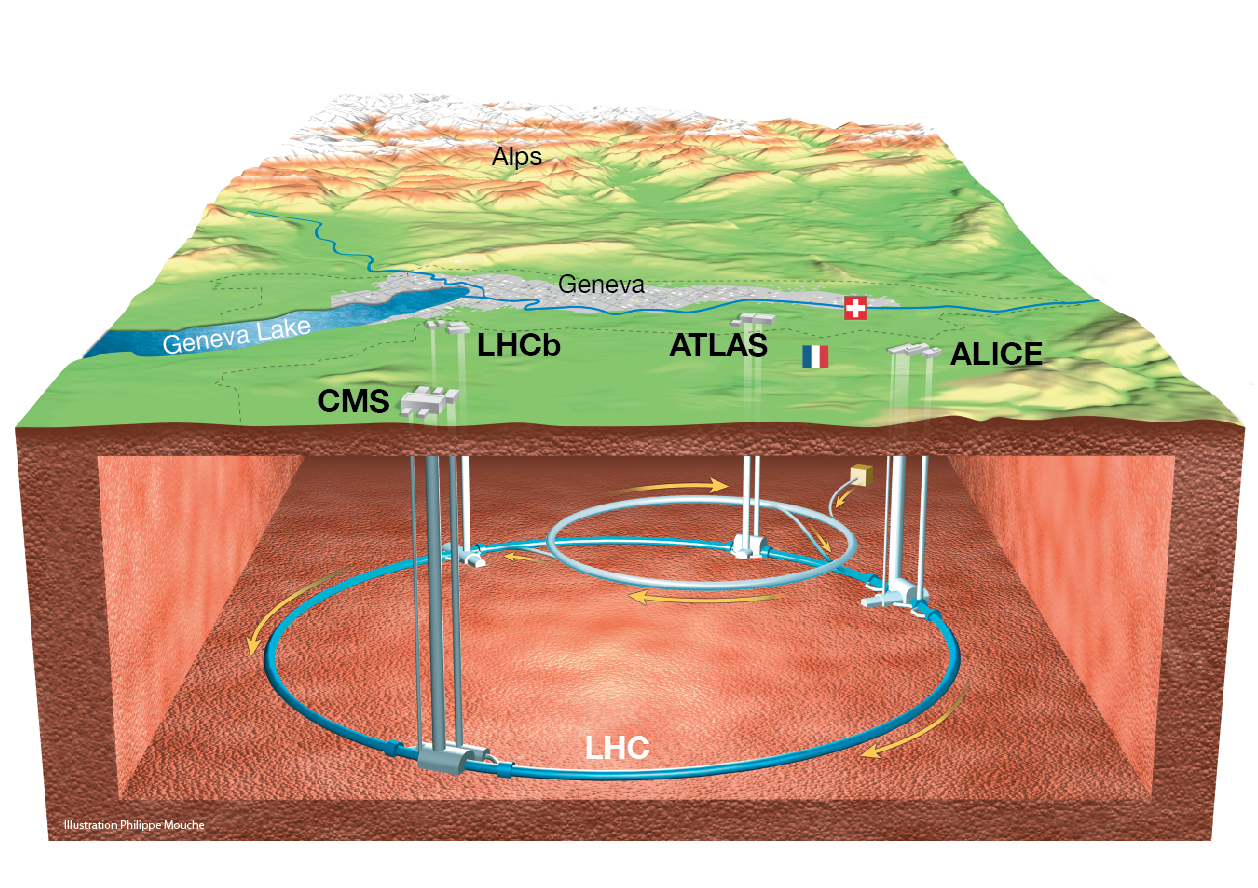
\includegraphics[width=0.75\linewidth]{plots/detector/LHC_overview.png}  \\
\caption[LHC overview]{The LHC and the four main experiments located at the four interaction regions.}
\label{fig:lhc-overview}
\end{figure}

The collider has four crossing points where the accelerated particles collide, as can be seen in the illustration in Figure~\ref{fig:lhc-overview}. Nine detectors have been constructed at the LHC, located underground in large caverns excavated at the LHC's intersection points. Two of them, the ATLAS experiment and \gls{cms}, are large general-purpose particle detectors. The other detectors have more specialized roles. ATLAS and CMS measure a variety of SM physics, such as Higgs boson and top quark measurements, as well as look for BSM physics.

Two of the most interesting parameters of a particle collider are the center-of-mass energy of the collisions, and the luminosity. Due to energy conservation, the higher the energy of the collision, the heavier a theoretical particle can be produced. Therefore, in order to probe more massive theoretical particles (such as DM candidates in SUSY), the higher collision energy is necessary. The second parameter is the luminosity. The instantaneous luminosity depends on machine parameters and is given by

\begin{equation}
\lumi=\frac{1}{\sigma} \dd{N}{t},
\end{equation}
where $\sigma$ is the corresponding cross section and $\ddinline{N}{t}$ is the rate of particle interactions. The integrated luminosity is given by integrating the instantaneous luminosity over a period of time
\begin{equation}
L=\int \lumi \rd .
\end{equation}
The number of expected events N for a given process can be expressed in terms of the corresponding cross section $\sigma$ times the integrated luminosity $L$
\begin{equation}
N=L \cdot \sigma.
\end{equation}
Therefore, for rare processes, \ie, processes with very low cross section $\sigma$, access to large enough number of produced events requires higher integrated luminosity $L$. The integrated luminosity recorded in run 2 in CMS was around $138 \fbinv$.

\section{The Compact Muon Solenoid experiment}
\label{sec:cms}

The Compact Muon Solenoid (CMS) experiment is one of two large general-purpose particle physics detectors built on the Large Hadron Collider (LHC) at CERN in Switzerland and France, as previously mentioned. The CMS apparatus has an overall length of 22\unit{m}, a diameter of 15\unit{m}, and weighs 14\,000 \unit{tonnes}. The central feature of the CMS apparatus is a superconducting solenoid of 6\unit{m} internal diameter, providing a magnetic field of 3.8\unit{T}. Within the solenoid volume are a silicon pixel and strip tracker, a lead tungstate crystal electromagnetic calorimeter (ECAL), and a brass and scintillator hadron calorimeter (HCAL), each composed of a barrel and two endcap sections. Forward calorimeters extend the pseudorapidity coverage provided by the barrel and endcap detectors. Muons are measured in gas-ionization detectors embedded in the steel flux-return yoke outside the solenoid. A more detailed description of the CMS detector, together with a definition of the coordinate system used and the relevant kinematic variables, can be found in Ref.~\cite{CMS:2008xjf}. A cutaway diagram of the CMS detector can be seen in Figure~\ref{fig:cms-detector}.

\begin{figure}[!htb]
\centering
\includegraphics[width=0.85\linewidth]{plots/detector/cms_detector.pdf}  \\
\caption[A cutaway diagram of the CMS detector]{A cutaway diagram of the CMS detector.}
\label{fig:cms-detector}
\end{figure}

Events of interest are selected using a two-tiered trigger system. The first level (L1), composed of custom hardware processors, uses information from the calorimeters and muon detectors to select events at a rate of around 100\unit{kHz} within a fixed latency of about 4\mus~\cite{CMS:2020cmk}. The second level, known as the high-level trigger (HLT), consists of a farm of processors running a version of the full event reconstruction software optimized for fast processing, and reduces the event rate to around 1\unit{kHz} before data storage~\cite{CMS:2016ngn}.

The global event reconstruction (also called particle-flow event reconstruction~\cite{CMS:2017yfk}) aims to reconstruct and identify each individual particle in an event, with an optimized combination of all subdetector information. In this process, the identification of the particle type (photon, electron, muon, charged hadron, neutral hadron) plays an important role in the determination of the particle direction and energy. Photons (\eg coming from \PGpz decays or from electron bremsstrahlung) are identified as ECAL energy clusters not linked to the extrapolation of any charged particle trajectory to the ECAL. Electrons (\eg coming from photon conversions in the tracker material or from \PB hadron semileptonic decays) are identified as a primary charged particle track and potentially many ECAL energy clusters corresponding to this track extrapolation to the ECAL and to possible bremsstrahlung photons emitted along the way through the tracker material. Muons (\eg from \PB hadron semileptonic decays) are identified as tracks in the central tracker consistent with either a track or several hits in the muon system, and associated with calorimeter deposits compatible with the muon hypothesis. Charged hadrons are identified as charged particle tracks neither identified as electrons, nor as muons. Finally, neutral hadrons are identified as HCAL energy clusters not linked to any charged hadron trajectory, or as a combined ECAL and HCAL energy excess with respect to the expected charged hadron energy deposit.

The energy of photons is obtained from the ECAL measurement. The energy of electrons is determined from a combination of the track momentum at the main interaction vertex, the corresponding ECAL cluster energy, and the energy sum of all bremsstrahlung photons attached to the track. The energy of muons is obtained from the corresponding track momentum. The energy of charged hadrons is determined from a combination of the track momentum and the corresponding ECAL and HCAL energies, corrected for the response function of the calorimeters to hadronic showers. Finally, the energy of neutral hadrons is obtained from the corresponding corrected ECAL and HCAL energies.

Jets are reconstructed offline from the energy deposits in the calorimeter towers, clustered using the anti-\kt algorithm~\cite{Cacciari:2008gp, Cacciari:2011ma} with a distance parameter of 0.4. In this process, the contribution from each calorimeter tower is assigned a momentum, the absolute value and the direction of which are given by the energy measured in the tower, and the coordinates of the tower. The raw jet energy is obtained from the sum of the tower energies, and the raw jet momentum by the vectorial sum of the tower momenta, which results in a nonzero jet mass. The raw jet energies are then corrected to establish a relative uniform response of the calorimeter in $\eta$ and a calibrated absolute response in transverse momentum \pt.

The primary vertex (PV) is taken to be the vertex corresponding to the hardest scattering in the event, evaluated using tracking information alone, as described in Section 9.4.1 of Ref.~\cite{CMS-TDR-15-02}. The missing transverse momentum vector \ptvecmiss is computed as the negative vector sum of the transverse momenta of all the PF candidates in an event, and its magnitude is denoted as \ptmiss~\cite{CMS:2019ctu}. The \ptvecmiss is modified to account for corrections to the energy scale of the reconstructed jets in the event.

The silicon tracker used in 2016 measured charged particles within the range $\abs{\eta} < 2.5$. For nonisolated particles of $1 < \pt < 10\GeV$ and $\abs{\eta} < 1.4$, the track resolutions were typically 1.5\% in \pt and 25--90 (45--150)\mum in the transverse (longitudinal) impact parameter~\cite{CMS:2014pgm}. At the start of 2017, a new pixel detector was installed~\cite{Phase1Pixel}; the upgraded tracker measured particles up to $\abs{\eta} < 3.0$ with typical resolutions of 1.5\% in \pt and 20--75\mum in the transverse impact parameter~\cite{DP-2020-049} for nonisolated particles of $1 < \pt < 10\GeV$.

Muons are measured in the pseudorapidity range $\abs{\eta} < 2.4$, with detection planes made using three technologies: drift tubes, cathode strip chambers, and resistive plate chambers. The single muon trigger efficiency exceeds 90\% over the full $\eta$ range, and the efficiency to reconstruct and identify muons is greater than 96\%. Matching muons to tracks measured in the silicon tracker results in a relative transverse momentum resolution, for muons with \pt up to 100\GeV, of 1\% in the barrel and 3\% in the endcaps. The \pt resolution in the barrel is better than 7\% for muons with \pt up to 1\TeV~\cite{CMS:2018rym}.


The integrated luminosities for the 2016, 2017, and 2018 data-taking years have 1.2--2.5\% individual uncertainties~\cite{CMS-LUM-17-003,CMS-PAS-LUM-17-004,CMS-PAS-LUM-18-002}, while the overall uncertainty for the 2016--2018 period is 1.6\%.

